\section{\textbf{Testes e análises do \textit{software}}}
\label{testes_do_software}
O \textit{software} criado no decorrer deste projeto é uma simples ideia de como usar técnicas de visão computacional aplicadas no reconhecimento de um jogador de futebol americano. Para exemplificar a usabilidade e os pontos fortes das técnicas utilizadas durante o desenvolvimento do mesmo, foram criadas várias situações para testar o desemprenho do algoritmo. Sendo assim, as figuras a seguir representam os testes feitos com o sistema desenvolvido.

\begin{figure}[ht]
	\caption{\label{fig_rec_numero}A imagem (A) representa os pontos de interesse encontrados nos números das camisas dos jogadores. A imagem (B) a sua identificaç ão.}
	\begin{center}
		\resizebox{1.0\linewidth}{!}{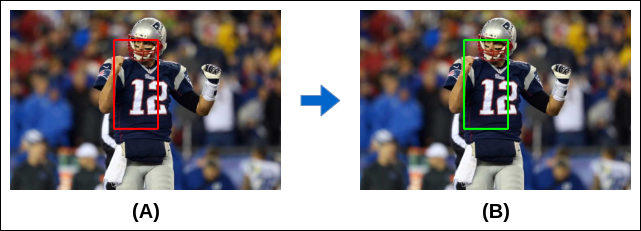
\includegraphics{6-Desenvolvimento-Projeto/imagens-desenvolvimento/representacao_numero.png}}
	\end{center}
	\centering \legend{Fonte: Elaborada pelos autores.}
\end{figure}

Inicialmente, o algoritmo foi testado em um cenário com imagens estáticas, como pode ser visto na \autoref{fig_comparativo_img} e \autoref{fig_rec_numero}, no qual ele analisa esta imagem, extraindo todos os seus padrões de características. Em seguida, ele realiza uma busca por similaridade na mesma imagem onde podemos notar, com maior evidência na  \autoref{fig_comparativo_img}, que mesmo ele cometendo alguns erros na parte de extração de características, a etapa de aprendizado de máquina entende os padrões e realiza  um balanceamento de quais característica são interessantes para serem levadas em consideração na hora de montar um modelo de busca. As características de menor interesse são dispensadas para reduzir a probabilidade do algoritmo cometer erros.

Em seguida, o algoritmo foi colocado em um cenário de análise de vídeo de uma partida de futebol americano. Nas etapas a seguir, o algoritmo utiliza o modelo de busca já treinado para identificar um jogador de futebol americano dentro de campo. Ou seja, não foi realizado nenhuma extração de característica de imagem, somente a técnica de busca por similaridade.

\begin{figure}[ht]
	\caption{\label{fig_rep_jogador_em_campo}Identificação de um jogador em uma partida de futebol americano.}
	\begin{center}
		\resizebox{.9\linewidth}{!}{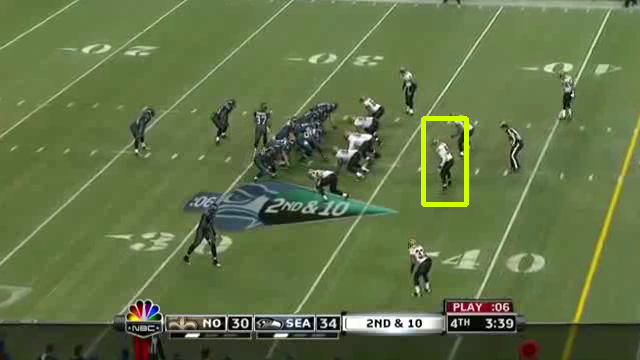
\includegraphics{6-Desenvolvimento-Projeto/imagens_teste/identificacao_jogador_em_campo_2.png}}
	\end{center}
	\centering \legend{Fonte: Elaborada pelos autores.}
\end{figure}

A \autoref{fig_rep_jogador_em_campo} foi retirada de um vídeo de uma partida de futebol americano. O algoritmo analisou \textit{frame} a \textit{frame} do vídeo para realizar a busca por similaridade seguindo o modelo de busca já treinado. Com base nessas informações, pode-se notar que o \textit{software} realizou uma leitura dos jogadores de futebol americano e identificou o jogador que mais se aproxima das características contidas no modelo de busca.

Outro fator que pode ser visto na \autoref{fig_rep_jogador_em_campo} é que o algoritmo identificou somente um jogador na cena analisada. Isso ocorre porque o comportamento seguido pelo \textit{software} e de analisar o jogador por inteiro e compará-lo com os padrões de características do modelo de busca, analisando também a sua fisionomia. Sendo assim, os outros jogadores podem ter atendido a algum ponto de característica contido dentro do modelo de busca, porém, aquele jogador identificado é o que mais se assimila ao modelo e por isso que ele foi identificado na cena.

\begin{figure}[ht]
	\caption{\label{fig_rep_jogador_mais_evidente}Identificação do jogador mais evidente.}
	\begin{center}
		\resizebox{.9\linewidth}{!}{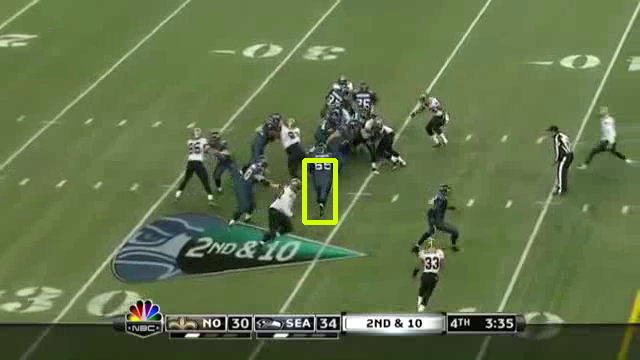
\includegraphics{6-Desenvolvimento-Projeto/imagens_teste/jogador_mais_evidente.png}}
	\end{center}
	\centering \legend{Fonte: Elaborada pelos autores.}
\end{figure}

Já na figura \autoref{fig_rep_jogador_mais_evidente} mostra a identificação do jogador mais evidente no ponto de vista do algoritmo. Como pode ser visto, no meio de uma jogada de futebol americano, o jogador que mais se encaixou nos padrões de características do modelo de busca foi identificado. Novamente, como citado na análise da \autoref{fig_rep_jogador_em_campo}, o algoritmo identificou somente um jogador dentre os demais, pois ele é o que mais se encaixa no modelo de busca.

Da mesma forma, a \autoref{fig_rep_jogador_em_movimento} representa a identificação de um jogador em movimento. Ao testar o \textit{software} nesse cenário, ele consegue, por um breve período, seguir o jogador analisado na sua corrida. Esse tempo não é o suficiente para analisar um jogador dentro de campo durante uma partida inteira, mas mostra que, com o aprimoramento do algoritmo e também o aprimoramento do modelo de busca, esse tipo de situação pode ser feita com mais eficiência.

\clearpage

\begin{figure}[ht]
	\caption{\label{fig_rep_jogador_em_movimento}Identificação de um jogador em movimento dentro de campo.}
	\begin{center}
		\resizebox{.7\linewidth}{!}{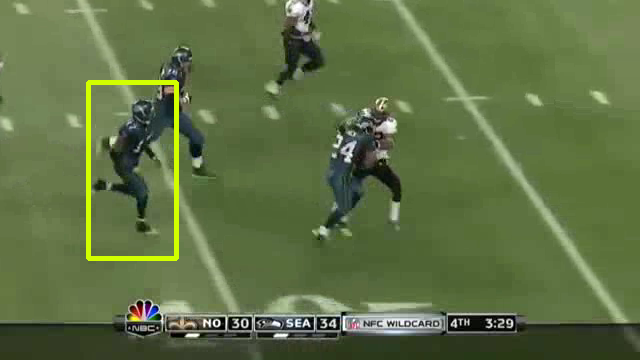
\includegraphics{6-Desenvolvimento-Projeto/imagens_teste/jogador_em_movimento.png}}
	\end{center}
	\centering \legend{Fonte: Elaborada pelos autores.}
\end{figure}

A \autoref{fig_rep_jogador_em_jogada} representa um jogador em uma velocidade mais alta do que o da \autoref{fig_rep_jogador_em_movimento}. Isso ocorreu devido a um lance que exigiu mais condicionamento físico do jogador de futebol americano. Mesmo nesse cenário, o algoritmo também foi capaz de identificar e perseguir o jogador dentro de campo por um intervalo de tempo. No entanto, o algoritmo teve um pouco mais de dificuldade para capturar todos os movimentos e realizar a identificação do  jogador devido o seu excesso de velocidade, não sendo possível persegui-lo durante um bom tempo ou ate mesmo quando entra em contato com o seu adversário.

\begin{figure}[ht]
	\caption{\label{fig_rep_jogador_em_jogada}Identificação de um jogador em movimento para disputar uma jogada.}
	\begin{center}
		\resizebox{.8\linewidth}{!}{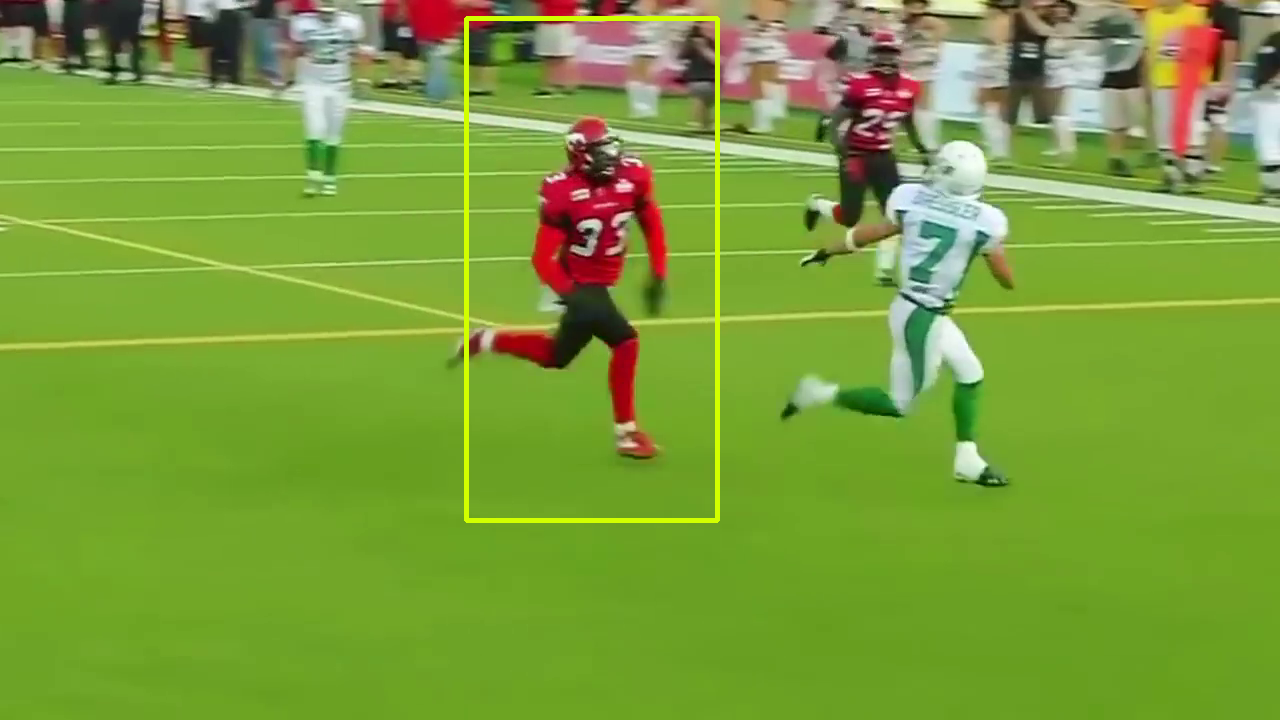
\includegraphics{6-Desenvolvimento-Projeto/imagens_teste/identificacao_jogadores_fa3.png}}
	\end{center}
	\centering \legend{Fonte: Elaborada pelos autores.}
\end{figure}

A \autoref{fig_rep_jogador_em_movimento_1} e \autoref{fig_rep_jogador_em_movimento_2} mostra como foi a tentativa do algoritmo de seguir um jogador em movimento para disputar uma jogada dentro de campo.

\begin{figure}[ht]
	\caption{\label{fig_rep_jogador_em_movimento_1}Tentativa de seguir os movimentos de um jogador dentro de campo.}
	\begin{center}
		\resizebox{.8\linewidth}{!}{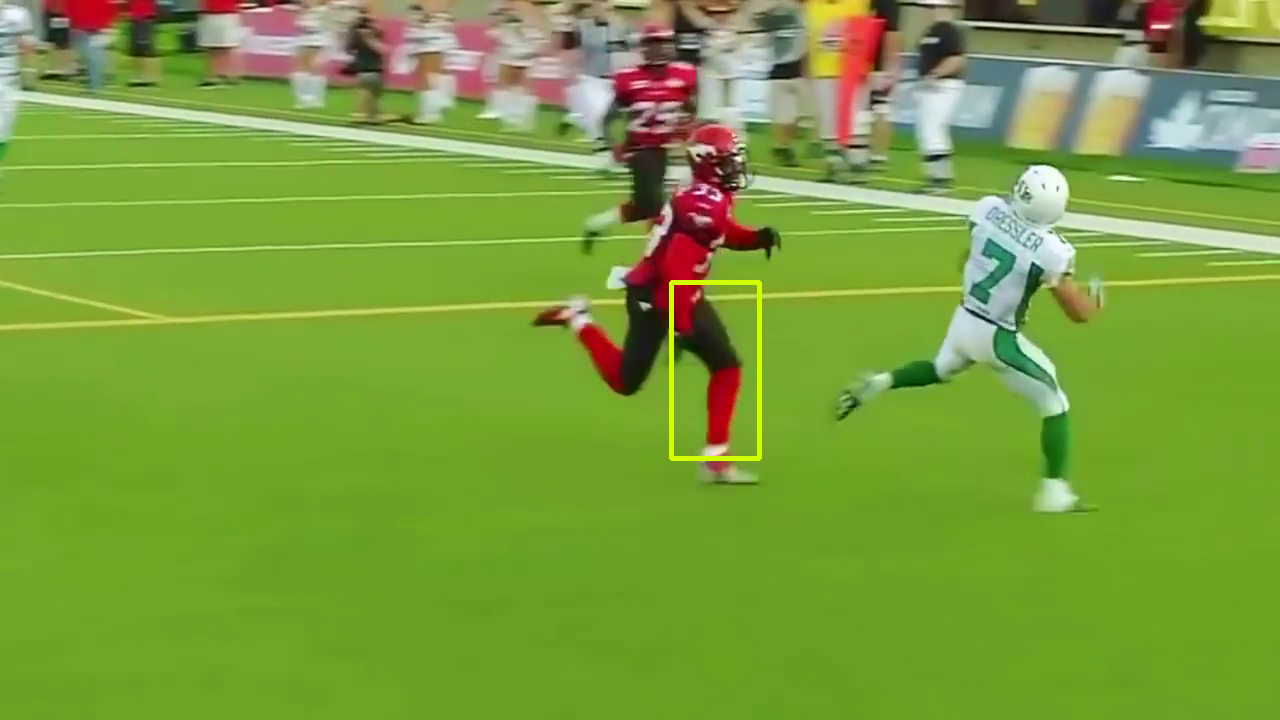
\includegraphics{6-Desenvolvimento-Projeto/imagens_teste/jogador_dentro_de_campo_1.png}}
	\end{center}
	\centering \legend{Fonte: Elaborada pelos autores.}
\end{figure}

\begin{figure}[ht]
	\caption{\label{fig_rep_jogador_em_movimento_2}Identificação do jogador de futebol americano após o movimento de corrida.}
	\begin{center}
		\resizebox{.8\linewidth}{!}{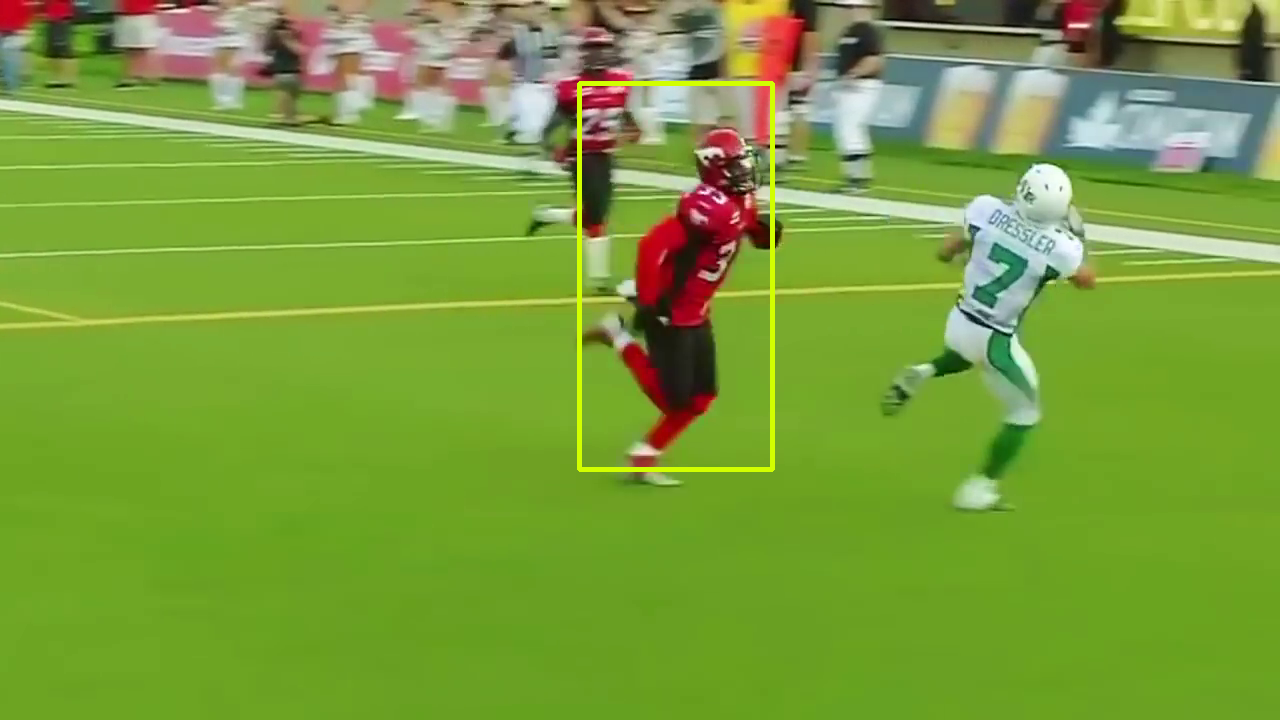
\includegraphics{6-Desenvolvimento-Projeto/imagens_teste/jogador_dentro_de_campo_9.png}}
	\end{center}
	\centering \legend{Fonte: Elaborada pelos autores.}
\end{figure}

Após a análise do \textit{frame} do vídeo representado pela \autoref{fig_rep_jogador_em_movimento_1}, no qual ele captura um movimento do jogador de futebol americano, foi feito a mesma análise utilizando o algoritmo que analisa imagens estáticas. A \autoref{fig_rep_erro} mostra que, dependendo da situação de movimento do jogador, o algoritmo não o reconhece, e sim reconhece o seu movimento. Isso ocorre porque a maioria das imagens que foram utilizadas para treinar o algoritmo continha jogadores de futebol americano em suas devidas situações dentro de campo, ou seja, os jogadores estavam correndo, em ataque, em disputa de bola e em várias outras situações de jogo. Sendo assim, os movimentos dos jogadores de futebol americano dentro de cambo também é um fator de análise do algoritmo e, consequentemente, é algo que pode interferir na identificação do mesmo.

\begin{figure}[ht]
	\caption{\label{fig_rep_erro}Identificação do movimento de um jogador de futebol americano.}
	\begin{center}
		\resizebox{.7\linewidth}{!}{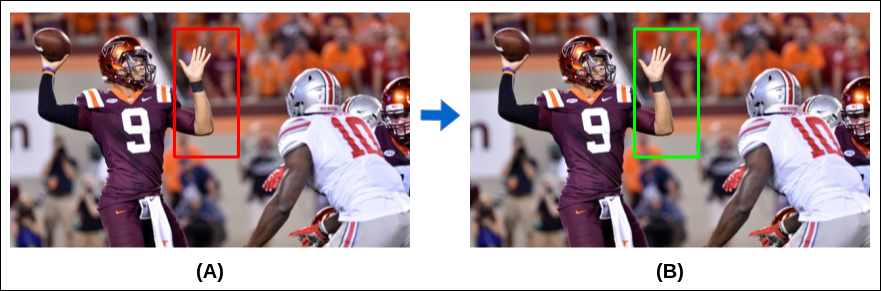
\includegraphics{6-Desenvolvimento-Projeto/imagens_teste/erro_algoritmo.png}}
	\end{center}
	\centering \legend{Fonte: Elaborada pelos autores.}
\end{figure}


A \autoref{fig_rep_dois_jogadores} representa basicamente o desempenho do algoritmo ao analisar o \textit{frame} do vídeo e identificar mais de um jogador de futebol americano dentro de campo. Como pode ser visto, o algoritmo conseguiu reconhecer dois jogadores dentro do \textit{frame} do vídeo, no entanto ele ainda não conseguiu identificar o restante. Nessa ocasião em específico, o algoritmo não seguiu com a identificação dos dois jogadores por um período longo e nem curto, pois ele “se perde” nas características e permanece identificando apenas um jogador.

\begin{figure}[ht]
	\caption{\label{fig_rep_dois_jogadores}Identificação de dois jogadores de futebol americano dentro de campo.}
	\begin{center}
		\resizebox{.7\linewidth}{!}{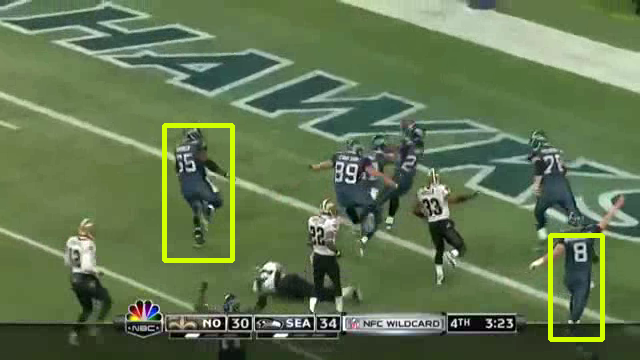
\includegraphics{6-Desenvolvimento-Projeto/imagens_teste/dois_jogadores_detectados.png}}
	\end{center}
	\centering \legend{Fonte: Elaborada pelos autores.}
\end{figure}

Já na \autoref{fig_rep_acessorios} podemos notar que o algoritmo não detectou nenhum jogador de futebol americano no \textit{frame} do vídeo. No entanto, como pode ser visto, o algoritmo conseguiu identificar alguns detalhes no uniforme dos jogadores. Isso ocorreu porque a variação de temperatura de cor naquela região atendeu aos padrões de características extraídas das imagens de treino que foram utilizadas para gerar o modelo de busca. Dessa forma, o algoritmo entendeu que, nesse \textit{frame} em especifico, os pontos de maior interesse que tem semelhança com o modelo de busca são os identificados na imagem.

\begin{figure}[ht]
	\caption{\label{fig_rep_acessorios}Identificação dos detalhes do uniforme de um jogador de futebol americano.}
	\begin{center}
		\resizebox{.8\linewidth}{!}{\includegraphics{6-Desenvolvimento-Projeto/imagens_teste/identificacao_jogadores_fa5.png}}
	\end{center}
	\centering \legend{Fonte: Elaborada pelos autores.}
\end{figure}

Outro fator muito interessante a ser analisado é a identificação feita pelo algoritmo na \autoref{fig_rep_arbitro}. Como pode ser visto, o sistema identificou o árbitro dentro de campo, e não  um dos jogadores de futebol americano. Essa situação foi bastante inusitada, pois não foi alterado nenhum parâmetro de busca e o modelo de busca também não foi alterado. Sendo assim, com base na \autoref{fig_rep_acessorios} e \autoref{fig_rep_arbitro}, pode-se concluir que a diferença de tonalidade dos uniformes também é um parâmetro que o algoritmo leva em consideração para realizar o processamento de imagem.

\clearpage

\begin{figure}[ht]
	\caption{\label{fig_rep_arbitro}Reconhecimento do árbitro dentro de campo.}
	\begin{center}
		\resizebox{.8\linewidth}{!}{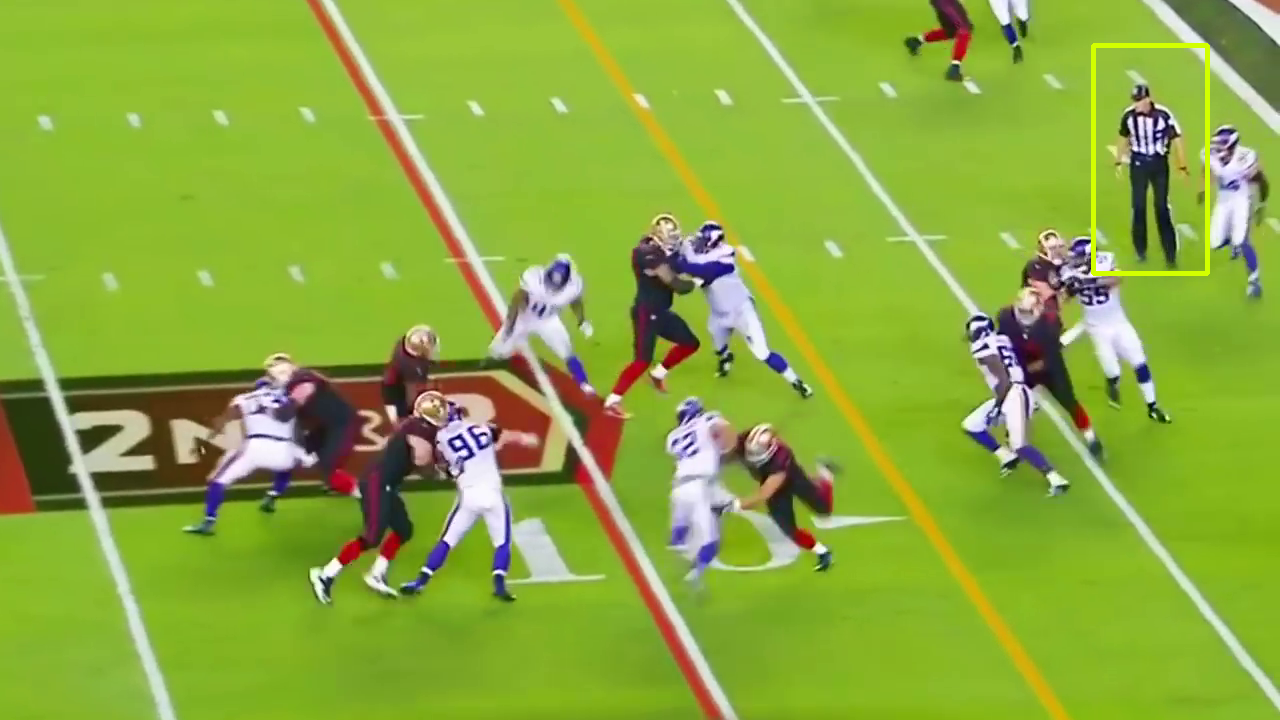
\includegraphics{6-Desenvolvimento-Projeto/imagens_teste/identificacao_arbitro.png}}
	\end{center}
	\centering \legend{Fonte: Elaborada pelos autores.}
\end{figure}

A \autoref{fig_processamento_maquina}  representa o consumo de \textit{hardware} quando executamos o algoritmo para realizar a análise de um vídeo. Como pode ser visto, o \textit{software} requer muito poder de processamento da máquina, consumindo grande parte dos seus recursos.  Vale lembrar que este teste foi bem simples e mostra superficialmente os recursos necessários para a execução do algoritmo. Na \autoref{novos_estudos} foi sugerido um estudo mais avançado sobre esse consumo de \textit{hardware}.

\begin{figure}[ht]
	\caption{\label{fig_processamento_maquina}Representação do processamento da máquina.}
	\begin{center}
		\resizebox{.7\linewidth}{!}{\includegraphics{6-Desenvolvimento-Projeto/imagens_teste/processamento_maquina.png}}
	\end{center}
	\centering \legend{Fonte: Elaborada pelos autores.}
\end{figure}

\clearpage